\section*{2. The Milky Way rotation curve}

Our Galaxy, the Milky Way, has a steeply rising rotational velocity near the center, but quickly flattens
out to $235 \frac{km}{s}$ (See figure below). By observing the density of stars in the Galaxy disk and
bulge we estimate a baryonic mass of $40 \cdot 10^9 M_{\circ}$ solar masses to be contained inside a 
Radius of 10 kpc.\\
\\
a) What would be the rotational velocity at 10 kpc if the Milky Way were composed of only the baryonic
matter in the bulge and the disk?\\
\\
We can calculate  the velocity with the following formula:
\begin{equation*}
  v = \sqrt{\frac{G \cdot M}{r}}
\end{equation*}
If we insert the given values and the gravitational constant $G$ we receive:
\begin{equation*}
  \begin{split}
    v &= \sqrt{\frac{4.302 \cdot 10^{-3} pc (\frac{km}{s})^2 \cdot \frac{1}{M_{\circ}} \cdot 40 \cdot 10^9 \cdot M_{\circ}}{10 kpc}}\\
      &= \sqrt{\frac{4.302 \cdot 10^{-3} pc (\frac{km}{s})^2 \cdot \frac{1}{M_{\circ}} \cdot 40 \cdot 10^9 \cdot M_{\circ}}{10,000 pc}}\\
      &= \sqrt{\frac{4.302 \cdot 10^{-3} (\frac{km}{s})^2 \cdot 40 \cdot 10^9}{10,000}}\\
      &= \sqrt{\frac{4.302 \cdot (\frac{km}{s})^2 \cdot 40 \cdot 10^6}{10,000}}\\
      &= \sqrt{\frac{4.302 \cdot (\frac{km}{s})^2 \cdot 4 \cdot 10^7}{10,000}}\\
      &= \sqrt{\frac{4.302 \cdot (\frac{km}{s})^2 \cdot 4 \cdot 10^3}{1}}\\
      &= \sqrt{4,302 \cdot (\frac{km}{s})^2 \cdot 4}\\
      &= \sqrt{17,208 \cdot (\frac{km}{s})^2}\\
      &\approx 131.1793 \frac{km}{s}
  \end{split}
\end{equation*}
b) Given that the true rotational velocity at 10 kpc is $235 \frac{km}{s}$, what mass of dark matter must
be contained in a halo of radius 10 kpc? What is the ratio of matter to dark matter at this radius?\\
\\
We expected a velocity of around $131 \frac{km}{s}$ but found a velocity of $235 \frac{km}{s}$. Therefore
we have a difference of $104 \frac{km}{s}$ for which the dark matter must be responsible. If we plug the
true velocity into the previous formula:
\begin{equation*}
  \begin{split}
    235 \frac{km}{s} &= \sqrt{\frac{4.302 \cdot 10^{-3} pc (\frac{km}{s})^2 \cdot \frac{1}{M_{\circ}} \cdot M}{10 kpc}}\\
    1 &= \sqrt{\frac{4.302 \cdot 10^{-3} pc (\frac{km}{s})^2 \cdot \frac{1}{M_{\circ}} \cdot M}{10 kpc}} \frac{1}{235 \frac{km}{s}}\\
    1 &= \sqrt{\frac{4.302 \cdot 10^{-3} pc (\frac{km}{s})^2 \cdot \frac{1}{M_{\circ}} \cdot M}{10 kpc}} \sqrt{\frac{1}{235^2 (\frac{km}{s})^2}}\\
    1 &= \sqrt{\frac{4.302 \cdot 10^{-3} pc (\frac{km}{s})^2 \cdot \frac{1}{M_{\circ}} \cdot M}{10 kpc} \frac{1}{235^2 (\frac{km}{s})^2}}\\
    1 &= \sqrt{\frac{4.302 \cdot 10^{-3} pc (\frac{km}{s})^2 \cdot \frac{1}{M_{\circ}} \cdot M}{10 kpc 235^2 (\frac{km}{s})^2}}\\
    1 &= \sqrt{\frac{4.302 \cdot 10^{-3} pc \cdot \frac{1}{M_{\circ}} \cdot M}{10 kpc 235^2}}\\
    1 &= \sqrt{\frac{4.302 \cdot 10^{-3} pc \cdot \frac{1}{M_{\circ}} \cdot M}{10,000 pc 235^2}}\\
    1 &= \sqrt{\frac{4.302 \cdot 10^{-3} \frac{1}{M_{\circ}} \cdot M}{10,000 \cdot 235^2}}\\
    1 &= \sqrt{\frac{4.302 \cdot 10^{-3} \frac{1}{M_{\circ}}}{10,000 \cdot 235^2}} \sqrt{M}\\
    \frac{1}{\sqrt{\frac{4.302 \cdot 10^{-3} \frac{1}{M_{\circ}}}{10,000 \cdot 235^2}}} &= \sqrt{M}\\
    \frac{1}{\frac{4.302 \cdot 10^{-3} \frac{1}{M_{\circ}}}{10,000 \cdot 235^2}} &= M\\
    \frac{10,000 \cdot 235^2}{4.302 \cdot 10^{-3} \frac{1}{M_{\circ}}} &= M\\
    \frac{10,000 \cdot 235^2 \cdot M_{\circ}}{4.302 \cdot 10^{-3}} &= M\\
    1.2837 \cdot 10^{11} \cdot M_{\circ} &\approx M
  \end{split}
\end{equation*}
This should be the mass within the 10 kpc radius if the body is moving at $235 \frac{km}{s}$. The 
difference of the masses is:
\begin{equation*}
  1.2837 \cdot 10^{11} \cdot M_{\circ} - 4 \cdot 10^{10} \cdot M_{\circ} = 8.837 \cdot 10^{10} \cdot M_{\circ}
\end{equation*}
The difference of the masses must be the mass of the dark matter, which causes the difference in velocity
received by the calculation and the true velocity. The ratio of dark matter to matter is therefore:
\begin{equation*}
  \begin{split}
    \frac{8.837 \cdot 10^{10} \cdot M_{\circ}}{4 \cdot 10^{10} \cdot M_{\circ}} &= \frac{8.837}{4}\\
                                                                                &= 2.20925
  \end{split}
\end{equation*}\\
\\
\noindent\makebox[\textwidth]{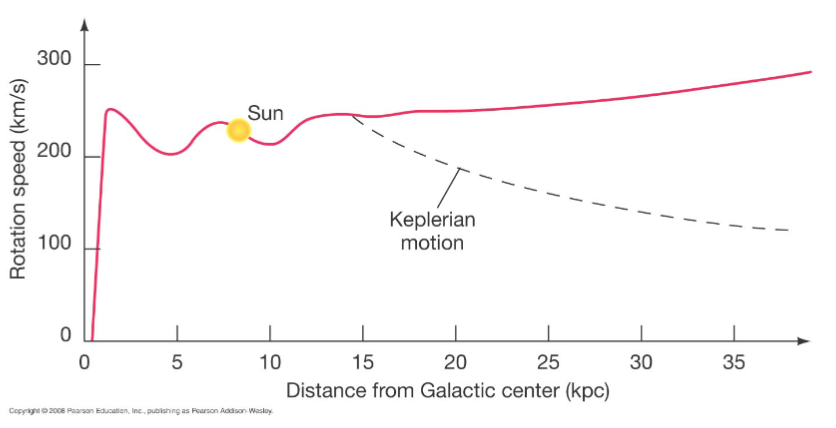
\includegraphics[scale=0.35]{velo.png}}\\
